\chapter{Mission Profile \& Ground Operations}
\label{ch:mission_profile}
\section{Mission Profile}
This chapter will construct the mission profile for an Urban Air Vehicle with Vertical Take-Off and Landing capabilities.
It must be considered that the take-off and landing configuration is different from the cruise configuration, so a transition between the two phases is necessary.
The mission profile (\Cref{fig:mission_profile}) consists of two main parts: the normal operational range (part A), and the emergency deviations (part B). Part A will be analysed first and more in-depth than part B, as part B depends on regulations, which currently are not in place for UAVs.

\begin{figure}[ht]
    \centering
    
\includegraphics[width=0.85\linewidth]{figures/Mission_Profile.pdf}
    \caption{Mission profile of the eVTOL aircraft}
    \label{fig:mission_profile}
\end{figure}

The mission starts with a vertical take-off from a vertiport in an urban area~\cite{scott2022vertiports}.
The aircraft then ascends vertically in the take-off configuration until it has gained enough altitude to transition, after which it will transition to the winged configuration.
Once in winged configuration, the aircraft will climb to the cruise altitude of around 500 meters.
The reason for climbing instead of vertically ascending is that it is better in terms of the degradation of the electrical system, because during vertical flight the aircraft has a thrust-to-weight ratio of more than 1, while winged climb has a ratio of around 0.4, depending on the aircraft~\cite{ADSEEIslides}.
Vertically ascending is more power-intensive than conventional climb, leading to higher engine wear and faster battery degradation.

After the climb phase, the aircraft will cruise in the conventional configuration.
In the cruise phase, more than 90\% of the horizontal distance will be covered.
The main parameter determining the cruise phase is the aircraft’s altitude. The cruise altitude for eVTOLs is a regulation that is not final yet but will likely be in the range of 500m ~\cite{kadhiresan2019conceptual}.

After the cruise, there are three options for landing, the first one being a regular descent, then a transition to VTOL configuration and a vertical landing, which is the standard scenario and the end of part A. Within part A, the distances might be longer due to weather; therefore, a 10\% operational reserve is considered to ensure the normal operating range is always met.

The two other options occur in part B, as they are emergency options when the landing area is temporarily or indefinitely obstructed.
In the first case, with temporary obstruction, the aircraft must wait until the vertiport is cleared again.
This can be done by either loitering in a winged configuration or hovering in a landing configuration.
Loitering is more energy efficient since the wings still provide lift. However, it does take up more airspace than hovering, which can be done in small airspace but takes a lot of power.

In the second scenario,
where the vertiport is indefinitely obstructed, the aircraft will need to land on a different vertiport,
meaning another climb, reroute, and descent is necessary.
This scenario is the one that defines the regulations of emergency reserves,
according to CS 23.25.a.2.i~\cite{easa_cs23_2020};
the aircraft should have enough power for continuous power operation for at least 45 minutes of extra flight,
which was deemed infeasible for eVTOLs with flight times of only 30 minutes by the eVTOL Flight Test Council~\cite{emergencyreserves}.
Therefore, the actual regulations for emergency power for eVTOLs are still being developed.
Furthermore, an article from TU Delft mentioned a loophole in the current electrical regulations~\cite{de2024new}.
For electrical aircraft, the emergency power unit does not need to be electric.
Therefore, from now on, it is assumed that a turbo generator will take care of the entire emergency reserve.

\section{Ground Operations}
Together with the mission profile, ground operations are here considered.
These shall be reduced to the bare minimum in order to make the in-between flight process as smooth as possible, facilitate the use of the vehicle, and reduce the Turn Around Time (TAT).

The option of re-charging the battery when at the vertiport, as well as at the vehicle's allocated parking space, is considered.
For efficient use, the eVTOL shall stay on the vertiport if use is expected within the next few hours and the vertiport is not needed by any other operator.
Should the in-between flights waiting time be longer, it shall be considered to park the vehicle somewhere else to minimise exposure to sun and/or bad weather.
This would also make the vertiport available to other operators to land on.
These operations might differ slightly in case a private vehicle and infrastructures are considered.
Similarly to what is done by \textcite{groundops}, \Cref{fig:GroundOps} shows the sequence of events just described.

\begin{figure}[h]
    \centering
    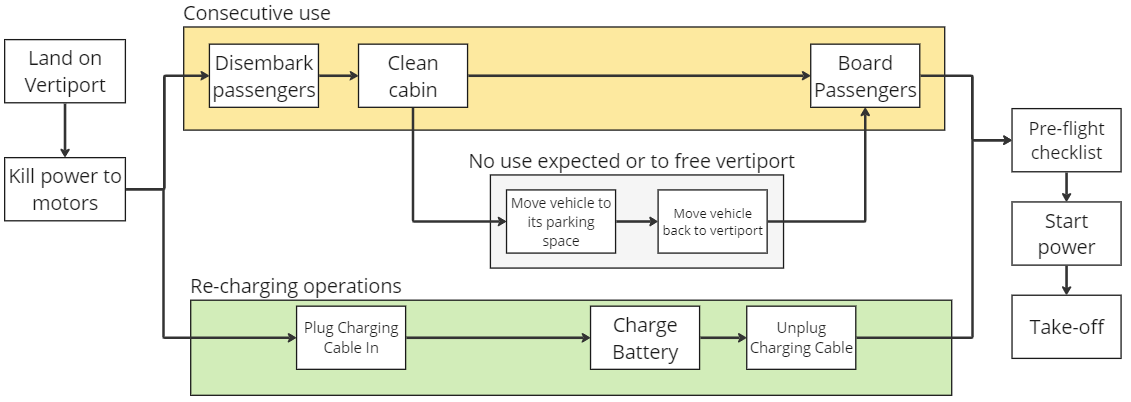
\includegraphics[width=\linewidth]{figures//Functions/GroundOps.png}
    \caption{Ground operations schematics of the eVTOL}
    \label{fig:GroundOps}
\end{figure}

